\documentclass[tikz,dvipsnames]{standalone}

\begin{document}

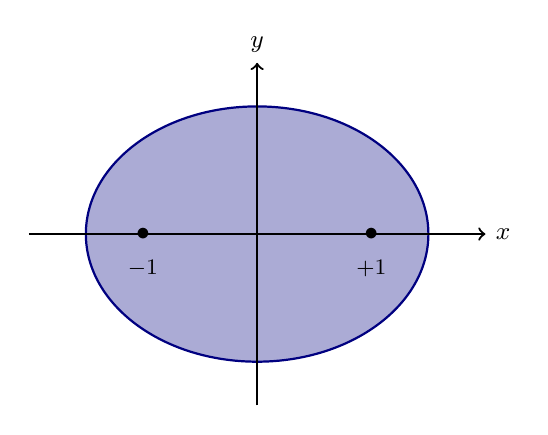
\begin{tikzpicture}[scale=1.45]
    \filldraw[color=NavyBlue,thick,fill=NavyBlue!55,fill opacity=0.6] (0, 0) ellipse (1.5cm and 1.118cm);
    \node[label=below:\footnotesize{$-1$}] (a) at (-1,0) {$\bullet$};
    \node[label=below:\footnotesize{$+1$}] (b) at (1,0) {$\bullet$};
    \draw[->,thick] (-2,0)--(2,0) node[right]{\small{$x$}};
    \draw[->,thick] (0,-1.5)--(0,1.5) node[above]{\small{$y$}};
    \end{tikzpicture}

\end{document}